\documentclass{article}
\usepackage[utf8]{inputenc}

\title{The \textit{abcd} of Interest Rate Basis Spreads}
\author{Ferdinando M. Ametrano, Luigi Ballabio, Paolo Mazzocchi}
\date{First version: November 2015\\
      This version: July 2016}

\usepackage{natbib}
\usepackage{graphicx}
\usepackage{lipsum}
\usepackage{amssymb} %per i simboli degli insiemi numerici
\usepackage{amsthm} %per \proof e \endproof
\usepackage{ragged2e} %giustifica
\justifying %giustifica
\usepackage{eurosym}
\usepackage{empheq}
\usepackage{xcolor}
\usepackage{amsmath}
\usepackage[T1]{fontenc}
%\usepackage[latin1]{inputenc}
\usepackage{lmodern}
\usepackage{hyperref}
\usepackage[titletoc,toc,title]{appendix}
\usepackage{subcaption}
\graphicspath{ {Figures/} }



\begin{document}

\maketitle

\begin{abstract}
    We show that forward rates can be modeled as \textit{abcd} parametric tenor basis spreads over the underlying overnight rate curve. This is possible for both continuously and simply compounded forward rates, with a simple approximation for converting between the corresponding basis. Increasing interest-rate tenor dominance, as empirically observed, is recovered and can be structurally enforced using a robust methodology improvement based on relative basis between the most liquid tenors. The smoothness requirement is moved from forward rate curves to tenor basis curves, properly dealing with the market evidence of jumps in forward rates. In the case of continuously compounded tenor basis, pseudo-discount factors are also available. An implementation of this methodology is available in the QuantLib open-source project.
\end{abstract}

%\tableofcontents





\noindent
This paper reports on a novel approach to interest-rate bootstrapping based on tenor basis spread \textit{abcd} parametrization.
It starts with a short introduction on recent developments and current best practices in a multi-curve world. Then, the rationale for smooth basis modeling is introduced. Equivalence between continuous and simple basis modeling is proved, and finally tenor-dominance relationships between interest-rate basis spreads are reproduced and built into the bootstrap approach. The EUR market case as of MMM dd yyyy is analyzed in detail, using the implementation of the proposed algorithms as available in the open-source QuantLib \cite{QuantLib} project.









\section{Rate Curves: Recent Developments and Current Best Practice}

[elaborate Henrard]

For a given tenor $x$ (e.g.,, 6 months, shortened in the following as 6M) we consider the simply compounded forward rates $F_x(t, t+x)$ (e.g., 6M Euribor, in the following shortened as $F_x(t)$): in a single-curve world their relation with discount factors $D(t)$ and instantaneous forward rates $f(t)$ is

\begin{equation}
1+F_x(t, t+x) \tau_x(t, t+x) = \frac{D(t)}{D(t+x)} = e^{\int_t^{t+x} f(u)\mathrm{d}u}
\end{equation}

where
\begin{itemize}
    \item $t$ is measured with an arbitrary monotonically increasing day-count convention (usually $Actual/365(Fixed)$) between the corresponding date $d$ and the settlement date $d_0$ corresponding to $t_0=0$ (where $D(0)=1$);
    \item $x$ can be ON, 1M, 3M, 6M, 1Y;
    \item $t+x$ is a shorthand for the time corresponding to the date $d_x=d+x$ which is a tenor $x$ later than the date $d$ corresponding to $t$ (according to all market and holiday conventions);
    \item $\tau_x(t, t+x)$ (in the following shortened as $\tau_x(t)$) is the year fraction between the dates $d$ and $d_x$ underlying the forward rate and measured according to its day-count convention $\tau_x$ (e.g., $Actual/360$ in the Euribor case).
\end{itemize}

Since the credit and liquidity crisis of summer 2007, large tenor basis spreads have been observed, implying that different rate curves are required for market-coherent estimation of forward rates with different tenors (e.g., ON Eonia, 1M Euribor, 3M Euribor, 6M Euribor, and 1Y Euribor). Ametrano and Bianchetti \cite{ametrano-bianchetti-1} have introduced the methodology for bootstrapping multiple forward rate curves using a set of plain vanilla market instruments \textit{homogeneous} in underlying rate tenor for each curve; however, their approach inherits from the single-curve world the calculation of forward rates as discount ratios, with their relation now becoming
\begin{equation}
\label{eq:ForwardAsPseudoDiscountRatio}
1+F_x(t) \tau_x(t) = \frac{D_x(t)}{D_x(t+x)} = e^{\int_t^{t+x} f_x(u) \mathrm{d}u}
\end{equation}
after the introduction of multiple forwarding curves represented by $D_x$ or alternatively $f_x$.

In this approach each forward-rate curve being bootstrapped was also used for discounting, in an endogenous way. Thus, once the forward curves were bootstrapped, using a single curve for actual cash-flow discounting would have led to prices not coherent with the forward estimation procedure.

The wide diffusion of bilateral collateral agreements and central clearing for interest rate derivatives has driven the adoption of the overnight curve for  discounting. The endogenous discounting used heretofore in forward curve bootstrapping was then replaced by exogenous discounting with the ON curve: this was consistent with the funding of market instruments in a finally coherent theoretical pricing framework for plain vanilla interest rate derivatives \cite{piterbarg, ametrano-bianchetti-2, mercurio}. In turn, this evolution has made clear that the discount factors $D_x$ used in equation \ref{eq:ForwardAsPseudoDiscountRatio} are just \textit{pseudo}-discount factors and should not be used for discounting cashflows.

% note: pseudo-discount useful in legacy systems

However, the calculation of forward rates from pseudo-discount factors has problems; the attempts to overcome them \cite{ametrano-mazzocchi, hagan, andreasen, ametrano-bianchetti-2, Burkard} have involved the introduction of synthetic values for $\{D_x(t), t<x \}$, research about suitable interpolation, careful selection of market instruments, dealing with negative rates, extreme slope changes in curves, and especially jumps (e.g., due to the turn-of-year effect). In the remainder of this paper, we will refer to the resulting pseudo-discount curves as \textit{legacy curves}.

For a while, we considered the possibility of bootstrapping forward rates directly. This would have solved some of the problems, but not all of them. Namely, jumps in the overnight curve translated to different amplitude jumps for longer tenor, each one to be estimated separately, and independent interpolation of forward curves still led to spurious oscillations in the implied tenor basis curves. Therefore we turned to the approach presented in the remainder of this paper, which provides an effective solution to these problems.








\section{Rationale for \textit{abcd} Smooth Basis Modeling}

We define the simple basis spread
\begin{equation}
\label{eq:S_x}
S_x(t) = F_x(t) - F_x^{ON}(t)
\end{equation}
as the difference between the simply-compounded forward rate $F_{x}(t)$ and an equivalent forward rate $F_{x}^{ON}(t)$ calculated on the ON curve over the same tenor $x$ by means of equation \ref{eq:ForwardAsPseudoDiscountRatio}.

Empirically, the basis can be parametrized as an \textit{abcd} function
\begin{equation}
\label{ABCD}
S_x(t) = (A_x + B_x t)e^{-C_x t} + D_x
\end{equation}
following Rebonato's notation \cite{rebonato}.

\begin{figure}[!ht]
\centering
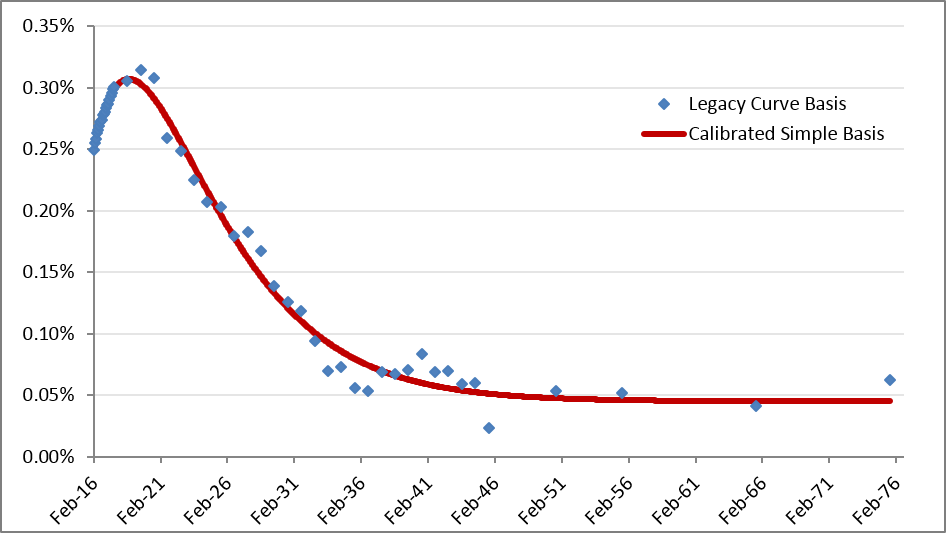
\includegraphics[width=0.9\textwidth]{Empirical6MBasis.png}
\caption{Calibrated 6M simple basis spread, plotted against the basis spreads calculated from the 6M and ON legacy curves.}
\label{Empirical6MBasis}
\end{figure}

In figure~\ref{Empirical6MBasis}, the parameters $a,b,c,d$ of $S_{6M}(t)$ were calibrated to obtain a best fit of the rates $F_{6M}(t) = F_{6M}^{ON}(t) + S_{6M}(t)$ to market rates. The basis spreads calculated from the 6M and ON legacy curves are plotted as reference; as mentioned earlier, it can be seen that they present spurious oscillations due to their interpolations changing convexity at different times. The market instruments used for calibration were a subset of those based on the 6M Euribor index, namely, FRAs and interest-rate swaps. [expand]

\begin{table}[p]
\centering
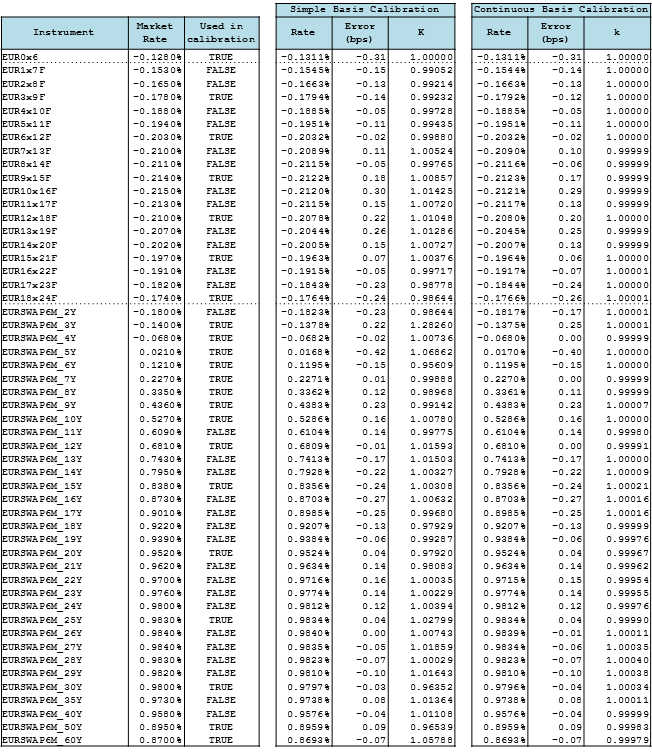
\includegraphics[width=1\textwidth]{6mBasisFit.png}
\caption{Results from calibration of simple and continuous 6M-ON basis spread.}
\label{6mBasisFit}
\end{table}

Obviously, a best-fit approach does not reprice market quotes exactly; in order to recover exact quotes we introduce, as in Rebonato \cite{rebonato}, a time-dependent correction factor $K_x(t)$.
In this case, the factor multiplies the calibrated forward rates $F_x^{calib}(t) = S_x(t) + F_x^{ON}(t)$ to obtain adjusted rates $$F_x^{adj}(t) = K_x(t) \cdot F_x^{calib}(t) = K_x(t) \cdot [S_x(t) + F_x^{ON}(t)].$$

The function $K_x(t)$ can be defined as the interpolation of a set of discrete factors $\left\{K_x(t_i)\right\}$. 
For instruments quoting a single forward rate (FRAs and futures), the $t_i$ is the fixing date of the rate and the correction factor can be easily calculated as
\begin{equation}
\label{direct-k}
K_x(t_i) = \frac{F_x^{mkt}(t_i)}{F_x^{calib}(t_i)}
\end{equation}
where $F_x^{mkt}(t_i)$ is the value of the contract quoted on the market and fixing at time $t_i$.

When dealing with swaps, whose quoted rates depend each on a number of forward rates, there is no direct formula giving the correction factor; however, it is a natural extension to use the fixing date of the last floating coupon as the pillar date $t_i$ and to obtain the corresponding $K_x(t_i)$ via root solving. For ease of implementation, the root-solving approach can also be used for FRAs and futures and leads to the same results as the direct formula (\ref{direct-k}).

The set of $K_x(t_i)$ is usually very close to 1; the results for our market case, obtained using linear interpolation between pillars, are shown in the ``simple basis calibration'' section of table~\ref{6mBasisFit} together with the corresponding errors.  The use of linear interpolation is a conservative choice that does not introduce spurious artifacts; the lack of discernible structure for the $K_x$ suggests that a more complex interpolation is not needed.

% note: why calibrate on just a subset?

% note: no pseudo-discount used or even available

% note: fit should be on prices, not rates










\section{Relation Between Continuous and Simple Basis}

% note: Although only the simple basis is observed in the market...

It has been argued \cite{schlenkrich-miemiec} that  for derivative pricing it is preferable to use the continuous basis spread
\begin{equation}
\label{eq:s_x}
s_x(t) = f_x(t) - f_{ON}(t),
\end{equation}
where $f_x(t)$ is the instantaneous forward rate on the $x$ curve and $f_{ON}(t)$ is the instantaneous forward rate on the ON curve. Moreover, a continuous basis provides well defined pseudo-discounts and will allow us to obtain tenor-basis dominance by construction, as explained in section \ref{sec:ensuring-tenor-dominance}.

We can find an approximated relationship between simple and continuous basis; we have that
\begin{equation}
1 + F_x(t) \tau_x(t) = e^{\int_t^{t+x} f_x(u) \mathrm{d}u}
\end{equation}
Since $f_x(t) = s_x(t) + f_{ON}(t)$, we have:
\begin{equation}
\begin{split}
1 + F_x(t) \tau_x(t) &= e^{\int_t^{t+x} [s_x(u) + f_{ON}(u)] \mathrm{d}u}\\
&= [1 + F_x^{ON}(t) \tau_x(t)]e^{\int_t^{t+x} s_x(u) \mathrm{d}u}.
\end{split}
\end{equation}
Therefore:
\begin{equation}
e^{\int_t^{t+x} s_x(u) \mathrm{d}u} = \frac{1+ F_x(t) \tau_x(t)}{1+ F_x^{ON}(t) \tau_x(t)}. 
\end{equation}
Taking the logarithms and using a first-order approximation, we have:
\begin{equation}
\label{simple-vs-continuous}
\begin{split}
\int_t^{t+x} s_x(u) \mathrm{d}u &= \ln{\left[\frac{1+ F_x(t) \tau_x(t)}{1+ F_x^{ON}(t) \tau_x(t)}\right]}\\ 
&\approx F_x(t) \tau_x(t) - F_x^{ON}(t)\\
&= S_x(t) \tau_x(t).
\end{split}
\end{equation}

When the simple basis is parametrized as an \textit{abcd} function, we find that the continuous basis can be approximated by a function of the same form and vice versa; to help distinguish the two, we'll use uppercase parameters $A_x, B_x, C_x, D_x$ for the simple basis and lowercase parameters $a_x, b_x, c_x, d_x$ for the continuous basis, just as we used $F_x(t)$ and $f_x(t)$ for the forward rates and $S_x(t)$ and $s_x(t)$ for the basis spreads.

Let us posit an \textit{abcd} parametrization for the continuous basis
\begin{equation}
s_x(t) = (a_x + b_x t)e^{-c_x t} + d_x;
\end{equation}
it follows that
\begin{equation}
\begin{split}
\int_t^{t+\tau_x} s_x(u) \mathrm{d}u &= \int_t^{t+\tau_x} \left[ (a_x + b_x u)e^{-c_x u} + d_x \right] \mathrm{d}u \\
                                     &= \left[\hat{A_x}(\tau_x) + \hat{B_x}(\tau_x) t\right] e^{-\hat{C}_x  t} + \hat{D_x}(\tau_x)
\end{split}
\end{equation}
with
\begin{equation}
\label{eq:integratedCoef}
\begin{split}
\hat{A_x}(\tau_x)&=-\left(\frac{a_x}{c_x}+ \frac{b_x}{c_x^{2}}+\frac{b_x}{c_x}\tau_x \right)e^{-c_x \tau_x}+\left(\frac{a_x}{c_x}+ \frac{b_x}{c_x^{2}}\right) \\
\hat{B_x}(\tau_x)&=\frac{b_x}{c_x}\left(1-e^{-c_x \tau_x}\right) \\
\hat{C_x}&=c_x \\
\hat{D_x}(\tau_x)&=d_x \tau_x.
\end{split}
\end{equation}
Substituting the above into equation~\ref{simple-vs-continuous}, we obtain
\begin{equation}
\left[\hat{A_x}(\tau_x) + \hat{B_x}(\tau_x) t\right] e^{-\hat{C}_x t} + \hat{D_x}(\tau_x) \approx S_x(t) \tau_x 
\end{equation}
and finally
\begin{equation}
S_x(t) \approx \left[\frac{1}{\tau_x}\hat{A_x}(\tau_x) + \frac{1}{\tau_x}\hat{B_x}(\tau_x) t\right] e^{-\hat{C}_x t} + \frac{1}{\tau_x}\hat{D_x}(\tau_x).
\end{equation}

Taking $\tau_x$ as constant\footnote{$\tau_x$ can assume almost constant values (namely $\tau_{6M}$ can be 0.5x with frequency 49\%, 0.5y with frequency 34\%, 0.5t with frequency x\%), its variations being easily absorbed in the overall approximation.}, the above is also an \textit{abcd} parametrization which compared to equation \ref{ABCD} gives the relationship
\begin{equation}
\begin{split}
A_x &\approx \frac{\hat{A_x}(\tau_x)}{\tau_x} 
    = \frac{1}{\tau_x} \left[ -\left(\frac{a_x}{c_x}+ \frac{b_x}{c_x^{2}}+\frac{b_x}{c_x}\tau_x \right)e^{-c_x \tau_x}+\left(\frac{a_x}{c_x}+ \frac{b_x}{c_x^{2}}\right) \right] \\
B_x &\approx \frac{\hat{B_x}(\tau_x)}{\tau_x} 
    = \frac{1}{\tau_x} \left[ \frac{b_x}{c_x}\left(1-e^{-c_x \tau_x}\right) \right]\\
C_x &\approx \hat{C}_x = c_x        \\
D_x &\approx \frac{\hat{D_x}(\tau_x)}{\tau_x} = d_x \\
\end{split}
\end{equation}
between the coefficients of the simple and continuous basis. Therefore, the parameters $A_x, B_x, C_x, D_x$ of the simple basis can be implied from the parameters $a_x, b_x, c_x, d_x$ of a calibrated continuous basis; alternatively the parameters $a_x, b_x, c_x, d_x$ of the continuous basis can be implied from the parameters $A_x, B_x, C_x, D_x$ of a calibrated simple basis. Table \ref{tab:6MBasisParam} shows that calibrations in the different simple/continuous domains for the 6M basis spreads provide comparable results when parameters are homogeneously compared.

\begin{table}
\centering
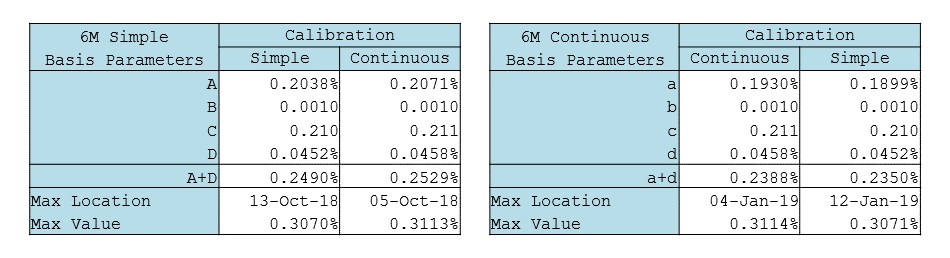
\includegraphics[width=0.9\textwidth]{6MSimple&ContBasisParam.png}
\caption{\textit{ABCD} and \textit{abcd} calibration parameters for the 6M basis spread curves.}
\label{tab:6MBasisParam}
\end{table}

The multiplicative correction factors $K_x(t_i)$ used to achieve exact repricing in the case of simple basis calibration cannot be converted to corresponding factors for the continuous basis calibration. Instead, multiplicative correction factors $k_x(t_i)$ can be bootstrapped and applied to the pseudo-discount factors that the continuous basis provides:
\begin{equation}
D_x^{adj}(t) = k_x(t) \cdot D_x^{calib}(t) = k_x(t) \cdot D_{ON}(t) \cdot e^{\int_0^{t} s_x(u) \mathrm{d}u}
\end{equation}
The adjusted discounts can then be used to retrieve forward rates as in:
\begin{equation}
F_x(t) = \frac{1}{\tau_x} \left[\frac{D^{adj}_x(t)}{D^{adj}_x(t+x)} - 1 \right]
\end{equation}

As before, the $k_x(t_i)$ are scattered around 1 without any relevant pattern or shape, suggesting linear interpolation as a safe choice. The continuous basis calibration results for the 6M market case are shown in table~\ref{6mBasisFit}; a chart is not provided, as is it practically identical to figure~\ref{Empirical6MBasis} (as implied by the very similar simple basis parameters in table~\ref{tab:6MBasisParam}).


\begin{figure}[t]
\centering
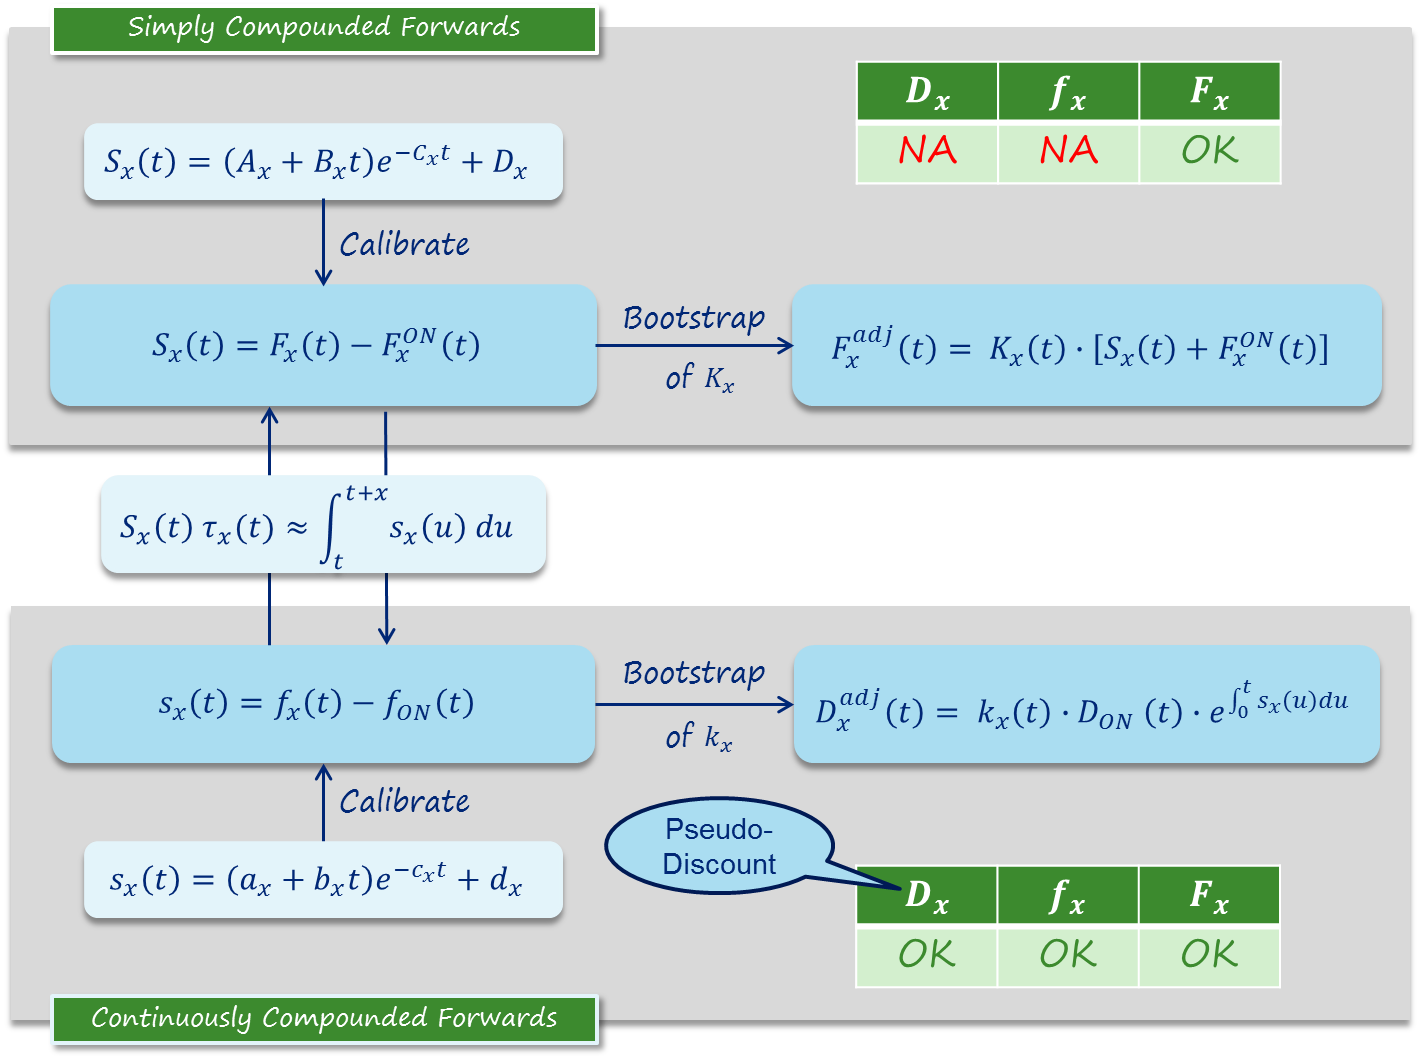
\includegraphics[width=0.9\textwidth]{SimpleContinuousEquivalence.png}
\caption{Equivalence between Simple and Continuous Basis.}
\label{SimpleContinuousEquivalence}
\end{figure}






\section{Comparison Between Tenors}
\label{sec:tenor-comparison}


Similar results can be obtained for the other tenors 1M, 3M, 1Y (see figures, tables...)

It is worth observing that the time $\tilde{T}$ corresponding to the maximum continuous spread is roughly the same for all tenors. If one considers the basis spread as a measure of uncertainty, being larger in period of stress and smaller when interbank risk is perceived to be negligible (to the point of being almost null before 2007), then $\tilde{T}$ is expected to be the same for all tenors. Instead, note that the location of the simple basis maximum is about half-tenor before the continuous basis one. This is to be expected, considering that the simple basis is the tenor-length moving-window integral of the continuous one: therefore, its maximum is largest when the maximum of the continuous spread is roughly in the center of the integration interval.
 
\begin{figure}[t]
\centering
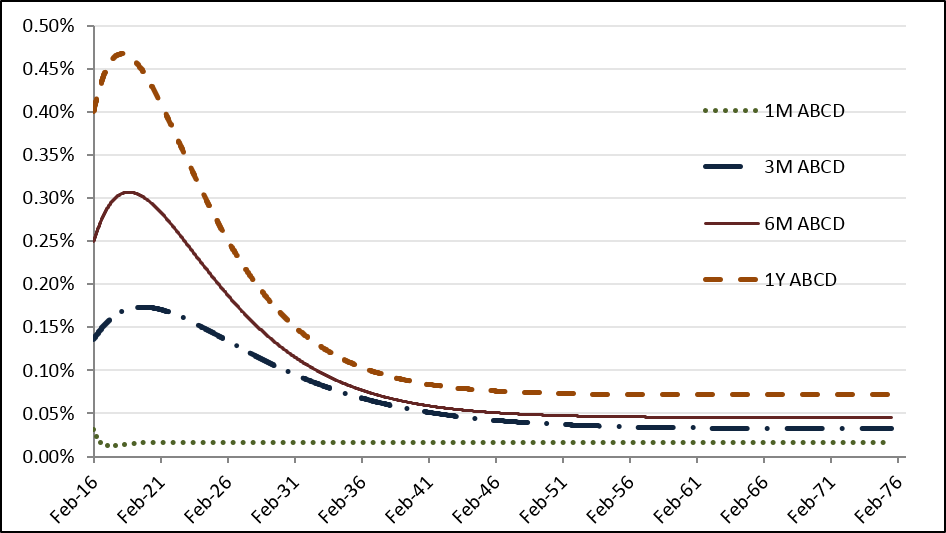
\includegraphics[width=0.9\textwidth]{SimpleBasis.png}\vfil
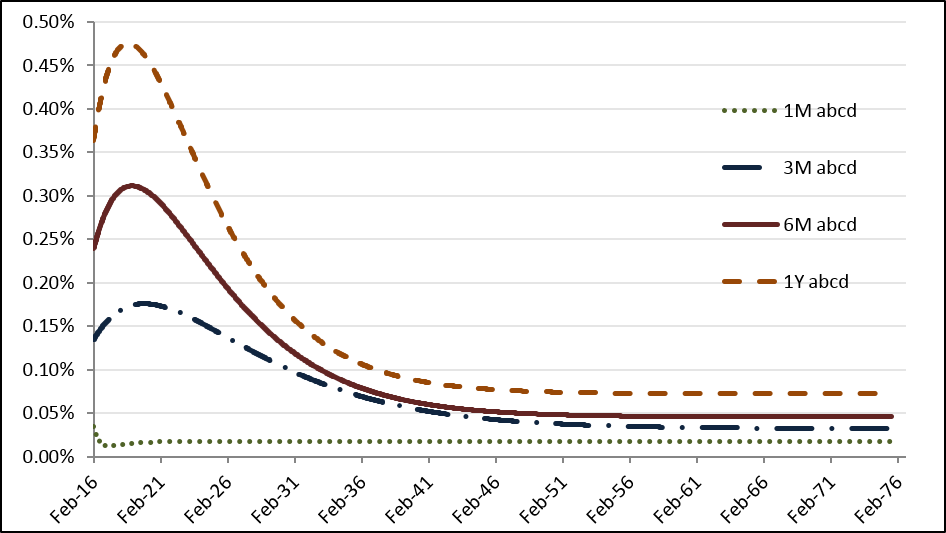
\includegraphics[width=0.9\textwidth]{ContinuousBasis.png}
\caption{Simple Basis (above) and Continuous Basis (below).}
\label{SimpleAndContinuousBasis}
\end{figure}

\begin{table}
\centering
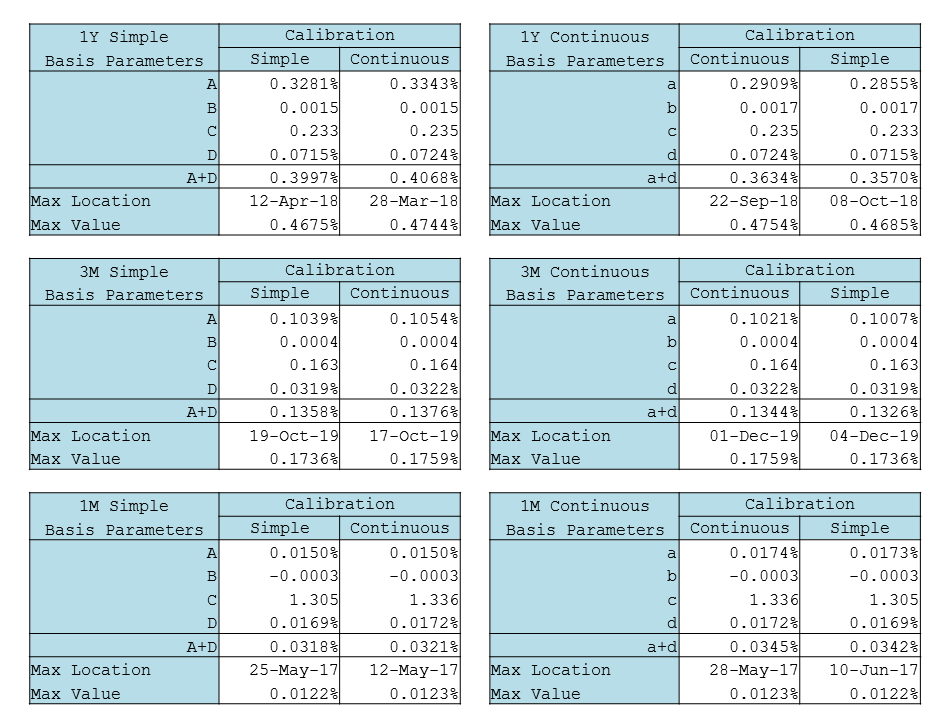
\includegraphics[width=0.9\textwidth]{Simple&ContBasisParam.png}
\caption{\textit{ABCD} and \textit{abcd} calibration parameters for 1M, 3M and 1Y basis spread curves.}
\label{tab:BasisParam}
\end{table}

\begin{table}[p]
\centering
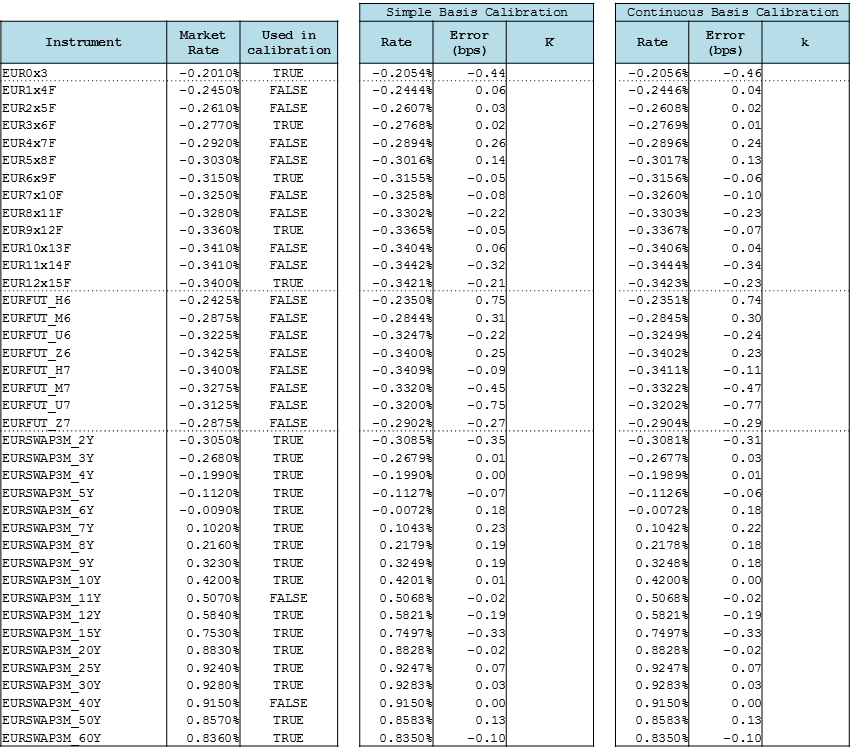
\includegraphics[width=1\textwidth]{3mBasisFit.png}
\caption{Results from calibration of simple and continuous 3M-ON basis spread.}
\label{3mBasisFit}
\end{table}

\begin{table}[p]
\centering
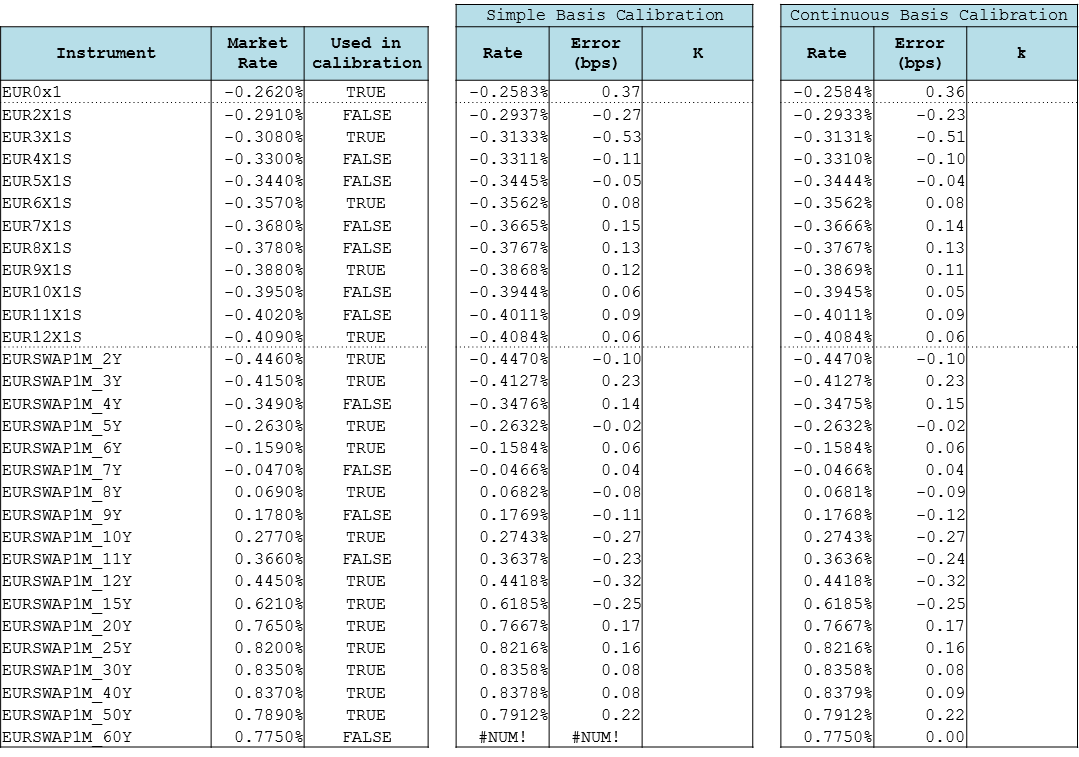
\includegraphics[width=1\textwidth]{1mBasisFit.png}\vfill
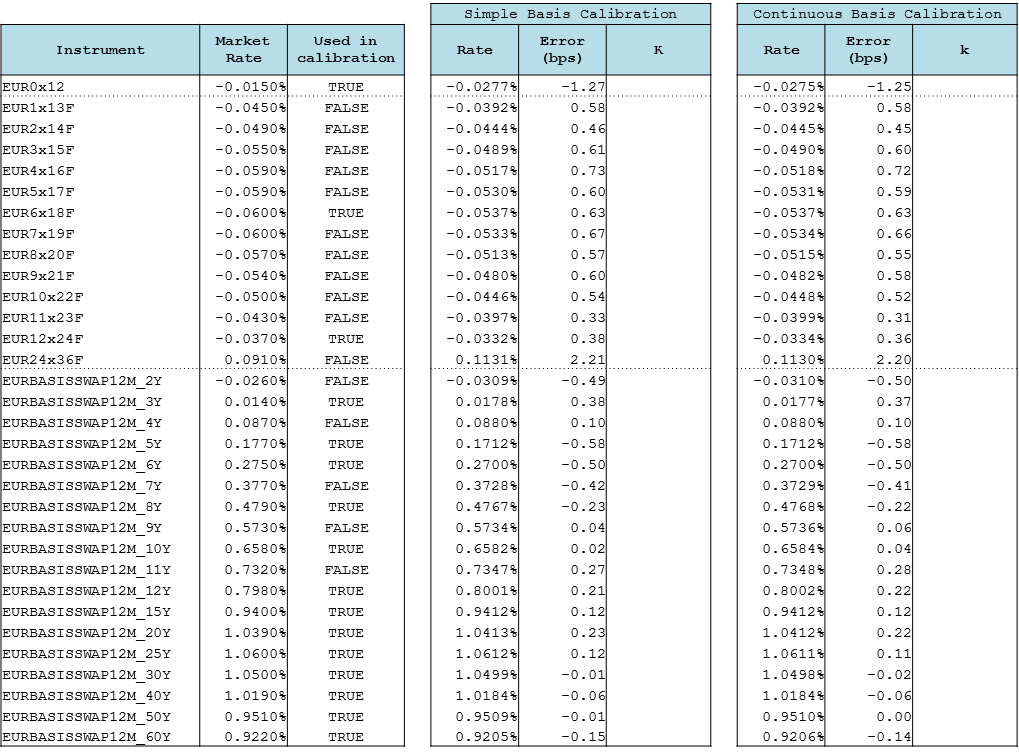
\includegraphics[width=1\textwidth]{1yBasisFit.png}
\caption{Results from calibration of simple and continuous: 1M-ON basis spread (above), 1Y-ON basis spread (below).}
\label{1mBasisFit}
\end{table}

1M being basically flat and very small the bid/ask noise is higher then the signal.

\section{Ensuring Tenor Dominance}
\label{sec:ensuring-tenor-dominance}

It is a comforting result of the previous section that tenor dominance is empirically retrieved: this should be expected, as longer tenors imply higher risks and therefore larger spreads. This point is so crucial that one might want to ensure it by construction. This can be achieved by calibrating basis spread between adjacent tenors $y<x$, generalizing equations \ref{eq:S_x} and \ref{eq:s_x} to:
\begin{equation}
\begin{split}
S_{x,y}(t) &= F_x(t) - F_x^{y}(t)\\
s_{x,y}(t) &= f_x(t) - f_{y}(t)
\end{split}
\end{equation}
with tenor $y$ taking the role of $ON$ and then applying the same approach illustrated in the previous sections.
Note that being the tenor $x$ in $F_x^{y}$ non-natural for a tenor $y$ curve, the tenor $y$ curve must provide pseudo-discounts to calculate such a forward rate. Therefore, the $y$ tenor must have been calibrated as continuous basis spread.

Unfortunately, the straightforward approach of calibrating the basis curves from lower to higher tenors in order (i.e., 1M over ON, 3M over 1M, 6M over 3M, and finally 1Y over 6M) is severely hampered by the reduced liquidity of the 1M tenor: the inferior quality of 1M calibration affects all subsequent steps.

Luckily, the problem can be solved by first calibrating the basis between the ON curve and the most liquid 6M tenor, and then switching to negative basis spread to calculate the 3M basis spread over 6M and the 1M over 3M, leaving only the 1Y basis to use positive spread over the 6M curve.  This gives good quality fits for the 6M, 3M and 12M curves, leaving only the 1M curve with a fit of lesser quality.

The results of this calculation are shown in figure...

\begin{figure}[t]
\centering
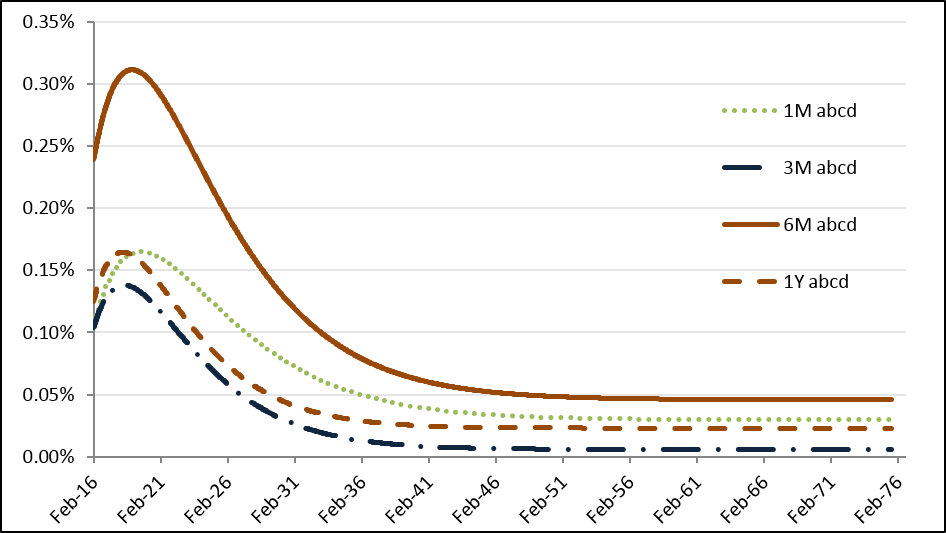
\includegraphics[width=0.9\textwidth]{TenorDominanceContinuousBasis.png}
\caption{.}
\label{TenorDominanceContinuousBasis}
\end{figure}



1M is even better as 1M over 3M, instead of 1M over ON:  See chart of 4 cont basis and C is almost the same. Same C means that a a difference of abcd is still an abcd



\section{Jumps}

see TOY jump on the 3M or 1M 

\section{Conclusion}

to be re-worded

We show that forward rates can be modeled as \textit{abcd} parametric tenor basis spreads over the underlying overnight rate curve. This is possible for both continuously and simply compounded forward rates, with a simple approximation for converting between the corresponding basis. Increasing interest-rate tenor dominance, as empirically observed, is recovered and can be structurally enforced. The smoothness requirement is moved from forward rate curves to tenor basis curves, properly dealing with the market evidence of jumps in forward rates. In the case of continuously compounded tenor basis, pseudo-discount factors are also available. An implementation of this methodology is available in the QuantLib open-source project.

Further research is 

financial parameters, financial constraints, nested calibration

proper modeling the ON curve is paramount, jumps included \cite{ametrano-mazzocchi}, \cite{ametrano-bertocchi}

synthetic deposit, especially 0x6, polynomial basis










\newpage
\appendix
\begin{appendices}
%  \renewcommand\thetable{\thesection\arabic{table}}
%  \renewcommand\thefigure{\thesection\arabic{figure}}
\section{Estimation of First Pillar}

In particular, for a given tenor $x$ in a multi-curve world the pseudo-discount factors for maturities below the forward tenor $\{D_x(t), t<x \}$ are not specified, even though forwards might depend on these 
pseudo-discounts: for instance, the 6M instruments (0x6, 1x7, 2x8, etc.) provide no information about the discount $D_{6M}(1M)$ used to estimate the $F_{6M}(1M)$ rate as
\begin{equation}
1+F_{6M}(1M) = \frac{D_{6M}(1M)}{D_{6M}(7M)} = \frac{e^{\int_0^{7M} f_{6M}(u)\mathrm{d}u}}{e^{\int_0^{1M} f_{6M}(u)\mathrm{d}u}}
\end{equation}
[elaborate why this is a problem]


\section{Derivation of Equivalence Formulas}

\subsection{\textit{abcd} parameterization}

In this section we assume that the continuous basis of tenor $x$ is an \textit{abcd} function. We have:
\begin{equation}
s_x(t) = (a + b t)e^{-c  t} + d
\end{equation}

Using the relationship between the continuous and the simple basis (\ref{SimpleContinuousBasis}), we can try to find the functional form of the simple basis. We have\footnote{here we are assuming that $\tau_x$ is constant.}:
\begin{equation}
S_x(t) \approx \frac{\int_t^{t+\tau_x} s(u) \mathrm{d}u}{\tau_x} = \frac{\int_t^{t+\tau_x} [(a + b u)e^{-c  u} + d] \mathrm{d}u}{\tau_x}
\end{equation}
Solving the integral, we have:
\begin{equation}
S_x(t) \approx \frac{[(A(\tau_x) + B(\tau_x) t)e^{-c  t} + D(\tau_x)]}{\tau_x}
\end{equation}
where
\begin{equation}\label{eq:integratedCoef}
\begin{split}
A(\tau_x)&=-\left(\frac{a}{c}+ \frac{b}{c^{2}}+\frac{b}{c}\tau_x \right)e^{-c\tau_x}+\left(\frac{a}{c}+ \frac{b}{c^{2}}\right) \\
B(\tau_x)&=\frac{b}{c}\left(1-e^{-c\tau_x}\right) \\
C(\tau_x)&= c \\
D(\tau_x)&=d\tau_x
\end{split}
\end{equation}
The last equation is fundamental; in fact we have that if the continuous basis ($s(t)$) is an \textit{abcd} function, even the simple basis ($S(t)$) is an \textit{abcd} function. Knowing the coefficients of the continuous basis we are able to calculate the coefficients of the simple basis ($a_{S_x},b_{S_x},c_{S_x},d_{S_x}$) in the following way: ($a,b,c,d$ are the coefficients of the continuous basis)
\begin{equation} \label{eq:simpleBasisCoef}
\begin{split}
a_{S_x}&=\left[-\left(\frac{a}{c}+ \frac{b}{c^{2}}+\frac{b}{c}\tau_x \right)e^{-c\tau_x}+\left(\frac{a}{c}+ \frac{b}{c^{2}}\right)\right]\frac{1}{\tau_x} \\
b_{S_x}&=\left[\frac{b}{c}\left(1-e^{-c\tau_x}\right)\right]\frac{1}{\tau_x} \\
c_{S_x}&= c \\
d_{S_x}&= d
\end{split}
\end{equation}

In this section we assume that the simple basis of tenor $x$ is an \textit{abcd} function. We have:
\begin{equation}
S_x(t) = (a_{S_x} + b_{S_x} t)e^{-c_{S_x}  t} + d_{S_x}
\end{equation}



\label{app:Polynomial parameterization}
\subsection{Polynomial parameterization} 
With \textit{polynomial parameterization} we refer to ($ n \in \mathbb{N}$):
\begin{equation}
f(t) = c_0 + c_1\cdot t + c_2\cdot t^2 + c_3\cdot t^3 + ... + c_n\cdot t^n = \sum_{i=0}^{n}(c_i \cdot t^i)
\end{equation}

This kind of parameterization replicate the behaviour of the basis (simple or continuous) in the first region, for maturities below 2 years typically.

In this section we assume that the continuous basis of tenor $x$ is a polynomial function of order $n$. We have:
\begin{equation}
s_x(t) = \sum_{i=0}^{n}(c_i \cdot t^i)
\end{equation}

Using the relationship between the continuous and the simple basis (\ref{SimpleContinuousBasis}), we can try to find the functional form of the simple basis. We have\footnote{here we are assuming that $\tau_x$ is constant.}:
\begin{equation}
S_x(t) \approx \frac{\int_t^{t+\tau_x} s_x(u) \mathrm{d}u}{\tau_x} = \frac{\int_t^{t+\tau_x} [\sum_{i=0}^{n}(c_i \cdot t^i)] \mathrm{d}s}{\tau_x}
\end{equation}
Solving the integral, we have that if the continuous basis is a polynomial of order $n$, than the simple basis is a polynomial of the same order\footnote{see appendix for details}.
Using the matrix notation, we have that the integrated coefficients are:

\begin{equation}
\begin{vmatrix} C_0(\tau_x) \\ C_1(\tau_x) \\ C_2(\tau_x) \\ \vdots \\ C_n(\tau_x) \end{vmatrix} = 
\begin{vmatrix}  
T_{(1,0)} \tau_x & \frac{1}{2}T_{(2,0)}\tau_x^2  & \frac{1}{3}T_{(3,0)}\tau_x^3  & \cdots & \frac{1}{n+1}T_{(n+1,0)}\tau_x^{n+1}  \\ 
0                & \frac{1}{2}T_{(2,1)}\tau_x    & \frac{1}{3}T_{(3,1)}\tau_x^2  & \cdots & \frac{1}{n+1}T_{(n+1,1)}\tau_x^{n+0}  \\
0                & 0                             & \frac{1}{3}T_{(3,2)}\tau_x    & \cdots & \frac{1}{n+1}T_{(n+1,2)}\tau_x^{n-1}  \\
\vdots           & \vdots                        & \vdots                        & \ddots & \vdots                                \\
0                & 0                             & 0                             & \cdots & \frac{1}{n+1}T_{(n+1,n)}\tau_x       
\end{vmatrix} 
\begin{vmatrix} c_0 \\ c_1 \\ c_2 \\ \vdots \\ c_n \end{vmatrix}
\end{equation}
Where $T_{(n,k)}$ is the binomial coefficient, i.e.:
\begin{equation}
T_{(n,k)} = \binom{n}{k}
\end{equation}
From now on we indicate the previous matrix with $\mathbf{A}$, the coefficients of the continuous basis with $\mathbf{c}$ and the coefficients of the simple basis with $\mathbf{c_{S_x}}$. We have:

\begin{equation} \label{eq:simplefromcontinuouspolynomial}
\mathbf{c_{S_x}} = \frac{1}{\tau_x} \mathbf{A} \cdot \mathbf{c}
\end{equation}

Here we parametrize the simple basis of tenor $x$ with a polynomial function of order $n$. We have:
\begin{equation}
S_x(t) = \sum_{i=0}^{n}(\mathbf{c_{S_x}}[i+1] \cdot t^i)
\end{equation}

Using the relationship between the continuous and the simple basis (\ref{SimpleContinuousBasis}), we can try to find the functional form of the continuous basis.
\begin{equation}
\int_t^{t+\tau_x} s_x(u) \mathrm{d}u \approx S_x(t) \tau_x= \tau_x \sum_{i=0}^{n}(\mathbf{c_{S_x}}[i+1] \cdot t^i) 
\end{equation}
We can use the result of the previous section, i.e. the continuous basis and simple basis are a polynomial of the same order. Inverting equation (\ref{eq:simplefromcontinuouspolynomial}), we have:
\begin{equation}
\mathbf{c} = \tau_x \mathbf{A}^{-1} \cdot \mathbf{c_{S_x}}
\end{equation}

\section{Properties of the abcd Function}



We now analyze the behaviour of the curve changing the parameters:

\begin{itemize}
\item \textbf{$c=0$}, we have:
\begin{equation}
f(t) = a + b\cdot t + d
\end{equation}
Therefore the parameterization becomes a line with angular coefficient equals to $b$ and the starting point, i.e. when $t=0$, equal to $a+d$.

\item $d$ is the long term value of the curve:
\begin{equation}
\lim_{t\rightarrow \infty} f(t)=d
\end{equation}

\item $a+d$ is the starting point of the curve:
\begin{equation}
\lim_{t\rightarrow 0} f(t)=a+d
\end{equation}

\item to find the max point we calculate the point where the first derivative is equal to $0$:
\begin{equation}
f(t)' = 0
\end{equation}

\begin{equation}
\begin{split}
f(t)'&= (a + b \cdot t) e^{-c \cdot t} \cdot(-c) + be^{-c \cdot t} \\
&= -c(a + b \cdot t) e^{-c \cdot t} + be^{-c \cdot t}\\
&= [-c(a + b \cdot t)+ b]e^{-c \cdot t}
\end{split}
\end{equation}
Therefore $t_{max}$:
\begin{equation}
\begin{split}
&[-c(a + b \cdot t_{max})+ b]e^{-c \cdot t} = 0 \\
&[-c(a + b \cdot t_{max})+ b] = 0 \\
&t_{max} = \frac{1}{c} -\frac{a}{b}
\end{split}
\end{equation}
And so the max point is equal to:
\begin{equation}
\begin{split}
f(t_{max})&= [a + b \cdot (\frac{1}{c} -\frac{a}{b})] e^{-c \cdot (\frac{1}{c} -\frac{a}{b})} + d \\
&= \frac{b}{c}e^{\frac{ac}{b} -1} + d
\end{split}
\end{equation}

\item in the first region, near $t=0$, we can approximate this parameterization using a quadratic function:
\begin{equation}
\begin{split}
f(t) &\sim (a + b\cdot t)(1- c \cdot t + o(t^2)) + d\\
&\sim (a - ac\cdot t +b - bc\cdot t^2 + o(t^2)) + d\\
&\sim a + b + d - ac\cdot t - bc\cdot t^2 + o(t^2)
\end{split}
\end{equation}

\item We now calculate the primitive $F$ of $f$. Since $f$ is substantially the product of two basic functions (one exponential and one polynomial) we will use integration by parts. We define

$$
g(t)=a + bt\ ,\ h(t)=-\frac{1}{c} e^{-ct}
$$

so that

$$
g^{\prime}(t)=b\ ,\ h^{\prime}(t)=e^{-ct}
$$

and calculate

\begin{equation}
\begin{split}
F(t)=\int f(t) \, \mathrm{d}t&=\int g(t)h^{\prime}(t) \, \mathrm{d}t + \int d \, \mathrm{d}t = \\
&=g(t)h(t) - \int g^{\prime}(t)h(t) \, \mathrm{d}t + dt + K=\\
&=-\frac{a + bt}{c}e^{-ct} + \frac{b}{c}\int e^{-ct} \, \mathrm{d}t + dt + K=\\
&=-\frac{a + bt}{c}e^{-ct} - \frac{b}{c^{2}}\int -ce^{-ct} \, \mathrm{d}t + dt + K=\\
&=-\frac{a + bt}{c}e^{-ct} - \frac{b}{c^{2}}e^{-ct} + dt + K =\\
&=-\left[\left( \frac{a}{c}+ \frac{b}{c^{2}}\right)+ \frac{b}{c} t\right]e^{-ct} + dt + K
\end{split}
\end{equation}

with $K\in{\mathrm{R}}$ constant.

\item The definite integral $G(t_{1},t_{2})$ of $f$ on a closed interval $[t_{1},t_{2}]$ is 

\begin{equation}
\begin{split}
G(t_{1},t_{2})&=F(t_{2})-F(t_{1})=\\
=&-\left[\left( \frac{a}{c}+ \frac{b}{c^{2}}\right)+ \frac{b}{c} t_{2}\right]e^{-ct_{2}} + dt_{2} + K +\\ 
&+\left[\left( \frac{a}{c}+ \frac{b}{c^{2}}\right)+ \frac{b}{c} t_{1}\right]e^{-ct_{1}} - dt_{1} - K
\end{split}
\end{equation}

If we now define $ \mathrm{d}t=t_{2}-t_{1},t=t_{1}$ we obtain
\begin{equation}
\begin{split}
G(t,t+\mathrm{d}t)&=-\left[\left( \frac{a}{c}+ \frac{b}{c^{2}}\right)+ \frac{b}{c}(t+\mathrm{d}t)\right]e^{-c t}e^{-c\mathrm{d}t}+\\ 
&+\left[\left( \frac{a}{c}+ \frac{b}{c^{2}}\right)+ \frac{b}{c} t\right]e^{-ct} + d\mathrm{d}t=\\
&=\left(A(\mathrm{d}t)+B(\mathrm{d}t)t\right)e^{-ct} + D(\mathrm{d}t)
\end{split}
\end{equation}
where
\begin{equation}
\begin{split}
A(\mathrm{d}t)&=-\left(\frac{a}{c}+ \frac{b}{c^{2}}+\frac{b}{c}\mathrm{d}t \right)e^{-c\mathrm{d}t}+\left(\frac{a}{c}+ \frac{b}{c^{2}}\right) \\
B(\mathrm{d}t)&=\frac{b}{c}\left(1-e^{-c\mathrm{d}t}\right) \\
D(\mathrm{d}t)&=d\mathrm{d}t
\end{split}
\end{equation}

Note that if $\mathrm{d}t$ is constant $G(t,t+\mathrm{d}t)\equiv G(t)$ is an abcd function with parameters $$A(\mathrm{d}t),B(\mathrm{d}t),c,D(\mathrm{d}t)$$

\end{itemize}

\section{ON Curve with Jumps} \label{app:ON Curve with Jumps}
The second critical point that we want to improve, is the $ON$ term structure: it is fundamental to build a good $ON$ curve, in order to obtain a correct estimation for $F_{on}$.

If we construct the $ON$ term structure using a cubic interpolation we obtain an oscillating curve.

To analyze this term structure in a better way we use a log-linear interpolation on Discount Factor.

Observing figure \ref{fig:ONtermstructureLinear} it seems that the $ON$ term structure has a lot of jumps, at least at the end of month.

To understand if our intuition is correct we observe the hystorical series of the \textit{Eonia} fixing. As we can see from figure \ref{fig:EONIAseries} has a jump at least at every end of month. Therefore any attempt to build a good term structure without consider jumps will fail.

We want to find a way to calculate the correct jumps' size using market available quotes. To achieve this result we can follow an approach similar to the one used by Burghardt \cite{Burghardt} to estimate turn of year jumps:
\begin{enumerate}
\item Construct an $ON$ curve using all liquid market quotes using a linear interpolation on log-discount factor;
\item Estimate the first jump assuming that a segment\footnote{$t_1$ = start date of the current segment and $t_2$ = end date of the current segment} out of line with preceding and following segments can be put back in line dumping the difference into the jump\footnote{$\tau_{Jump}$ is the year fraction between jump business day and the next business day}. For this reason we interpolate the value of the segment that includes a jump using the following or precending segment that not contain jump:
        \begin{equation}
        [F^{original}(t_1,t_2) - F^{interp}(t_1,t_2)] \cdot \tau(t_1,t_2) = Jump \cdot \tau_{Jump}
        \end{equation}
        \begin{equation}
        Jump = [F^{original}(t_1,t_2) - F^{interp}(t_1,t_2)]\cdot \frac{\tau(t_1,t_2)}{\tau_{Jump}}
        \end{equation}
\item Clean the curve from the jump at point 2
\end{enumerate}

We need to iterate 2 and 3 for every jump date. 







\end{appendices}


\bibliographystyle{plain}
\bibliography{main}{}

\end{document}
